\documentclass[a4paper]{article}
\usepackage[utf8]{inputenc}
\usepackage{lmodern}
\usepackage[T1]{fontenc}
\usepackage[portuguese,brazil]{babel}
\usepackage{url}
\usepackage{listings}
\usepackage{color}
\usepackage{textcomp}
\usepackage{pdfpages}
\usepackage{fancyvrb}
\usepackage{enumerate}
\usepackage{alltt}
\usepackage{array}
\usepackage{slashbox}
\usepackage{subfigure}
\usepackage[table]{xcolor}
%\usepackage[pdf]{pstricks}
%\usepackage{auto-pst-pdf}
%\usepackage{icomma} % para vírgula decimal / decimal comma
\definecolor{listinggray}{gray}{0.9}
\definecolor{mediumgray}{rgb}{0.6,0.6,0.6}
\definecolor{lbcolor}{rgb}{0.9,0.9,0.9}
\lstset{
    backgroundcolor=\color{lbcolor},
    tabsize=4,
    rulecolor=,
    basicstyle=\scriptsize,
    upquote=true,
    aboveskip={1.5\baselineskip},
    columns=fixed,
    showstringspaces=false,
    extendedchars=true,
    breaklines=true,
    prebreak = \raisebox{0ex}[0ex][0ex]{\ensuremath{\hookleftarrow}},
    frame=single,
    showtabs=false,
    showspaces=false,
    showstringspaces=false,
    identifierstyle=\ttfamily,
    keywordstyle=\color[rgb]{0,0,1},
    commentstyle=\color[rgb]{0.133,0.545,0.133},
    stringstyle=\color[rgb]{0.627,0.126,0.941},
}
\definecolor{pinegreen}{RGB}{0,139,114}
\definecolor{pgr}{RGB}{0,139,114}

\definecolor{aquamarine}{RGB}{0,181,190}
\definecolor{aqm}{RGB}{0,181,190}

\definecolor{skyblue}{RGB}{100,227,251}
\definecolor{skb}{RGB}{100,227,251}

\definecolor{pnk}{RGB}{255,150,150}

\newcommand{\comment}[1]{{\color{structure.fg!70!white}\footnotesize #1}}

\newcommand{\WD}[1]{\fbox{#1}\hspace{-0.5pt}}
\newcommand{\FWD}[1]{%
\fbox{%
\vbox to 10pt{\vfil%
\hbox to 0.8cm{\hfill#1\hfill}%
\vfil}%
}\hspace{-0.5pt}%
}

\def\bo{\mbox{\raise .35em \hbox{\underline{\scriptsize o}\ }}}
\def\ba{\mbox{\raise .35em \hbox{\underline{\scriptsize a}\ }}}

\def\A{\texttt{A}}
\def\B{\texttt{B}}
\def\C{\texttt{C}}
\def\D{\texttt{D}}
\def\E{\texttt{E}}
\def\F{\texttt{F}}

\title{Projeto de Máquinas de Estado}
\author{Organizado por Rodrigo Hausen. Original de Thomas L. Floyd.}
\date{Versão 0: \today}

\newcommand{\Not}[1]{\overline{#1}}
\def\And{\,}

\begin{document}

\maketitle

\vspace{-1cm}

\begin{center}
\url{http://compscinet.org/circuitos}
\end{center}

\begin{abstract}
Grande parte deste texto, exemplos e estrutura geral foram retirados
da seção 8-4 do livro \emph{Sistemas Digitais} (9a. ed.) de Thomas L. Floyd.
Este texto foi organizado para apresentar uma abordagem mais simples
para o projeto de máquinas de estados do que a contida no original.
\end{abstract}

\section{Modelo Geral de uma Máquina de Estados}

Antes de procedemos com qualquer técnica de projeto de contadores,
começaremos com uma definição geral de uma \emph{máquina de estados}:
um circuito sequencial genérico que consiste de uma seção feita a
partir de lógica combinacional e uma seção de memória (flip-flops),
como demonstrado na Figura~\ref{fig:modelo_geral}. Em um circuito
sequencial síncrono (que recebe um único sinal de \emph{clock}), há
uma entrada para o \emph{clock} na seção de memória como indicado.

\begin{figure}[!htp]
\begin{center}
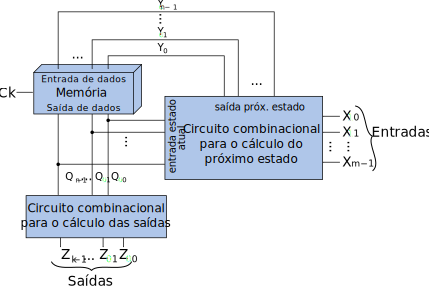
\includegraphics{images/state_machine_general}
\caption{Modelo geral de uma máquina de estados com entrada de \emph{clock}}
\label{fig:modelo_geral}
\end{center}
\end{figure}

A informação armazenada na seção de memória, assim como nas entradas
$X_0, X_1, \ldots X_{m-1}$ do circuito combinacional, é necessária para
a operação adequada do circuito. Em um dado instante, a memória está
em um estado denominado \emph{estado atual}, e avançará para o
\emph{próximo estado}, ao detectar uma transição do clock, de acordo
com as condições das linhas de ativação $Y_0, Y_1, \ldots, Y_{n-1}$.
O estado atual da memória é representado pelas variáveis de estado
$Q_0, Q_1, \ldots, Q_{n-1}$. Estas variáveis de estado determinam as
saídas do sistema $Z_0, Z_1, \ldots, Z_{k-1}$.

Nem todas as máquinas de estado possuem variáveis de entrada e
saída como neste modelo geral recém-discutido. Porém, todos possuem
variáveis de ativação e de estado. Contadores são um caso especial
de máquina de estado sensíveis à transição do clock. Nesta seção, um
procedimento geral de projeto de máquinas de estado é aplicado aos
contadores síncronos em uma série de passos.

\section{Exemplo: Implementação de Contador Gray}
Um código de Gray é um sistema
de numeração binário onde dois valores sucessivos diferem de apenas um bit.

Por exemplo, em um código de Gray de $3$ bits, a sequência de
numerais que representa os números de $0$ a $7$ é:
$000$, $001$, $011$, $010$, $110$, $111$, $101$, $100$.

\subsection{Passo 1: Diagrama de Estados}

O primeiro passo no projeto de um contador é a criação de um diagrama
de estados. Um \emph{diagrama de estados} mostra a progressão dos estados
através dos quais o contador avança a cada transição do clock.

A figura~\ref{fig:gray_state_diagram} é o diagrama de estados
para um contador de código de Gray
de $3$ bits. Este circuito particular possuirá apenas uma entrada, o clock,
e as únicas saídas serão aquelas obtidas dos estados dos flip-flops no
contador.

\begin{figure}[!htp]
\begin{center}
\includegraphics{images/gray_counter_states}
\caption{Diagrama de estados para um contador de Gray de $3$ bits.}
\label{fig:gray_state_diagram}
\end{center}
\end{figure}

\subsection{Passo 2: Tabela de transição}

Uma vez que o funcionamento da máquina de estados esteja definido
por meio de um diagrama de estado, o segundo passo é determinar uma
\emph{tabela de transição} para o próximo estado, que lista cada
estado do contador (estado atual), junto com o próximo estado
correspondente. \emph{O próximo estado é o estado para onde o
contador vai ao detectar uma transição do clock}.  A tabela de transição
é derivada do diagrama de estados. A Tabela~\ref{tab:gray} mostra
a tabela de transição para o contador de Gray de $3$ bits; $Q_0$
é o bit menos significativo.

\begin{table}[!htp]
\begin{center}
\caption{Tabela de transição para o contador de Gray de $3$ bits.}
\label{tab:gray}
\begin{tabular}{|ccc||ccc|}
\hline
\multicolumn{3}{|c||}{atual} &
\multicolumn{3}{c|}{próximo} \\
$Q_2$ & $Q_1$ & $Q_0$  & $Y_2$ & $Y_1$ & $Y_0$ \\
\hline
  0   &   0   &   0    &   0   &   0   &   1   \\ 
  0   &   0   &   1    &   0   &   1   &   1   \\ 
  0   &   1   &   1    &   0   &   1   &   0   \\ 
  0   &   1   &   0    &   1   &   1   &   0   \\ 
  1   &   1   &   0    &   1   &   1   &   1   \\ 
  1   &   1   &   1    &   1   &   0   &   1   \\ 
  1   &   0   &   1    &   1   &   0   &   0   \\ 
  1   &   0   &   0    &   0   &   0   &   0   \\
\hline
\end{tabular}
\end{center}
\end{table}

\subsection{Passo 3: determinação e otimização de expressões}

Usaremos uma memória composta por flip-flops do tipo D,
onde as linhas de ativação $Y_0$, $Y_1$, $Y_2$ determinarão
o próximo estado da saída de cada flip-flop. Para calcular
o estado de cada linha de ativação, precisamos determinar
uma expressão para cada variável $Y_i$ com base em
$Q_2$, $Q_1$ e $Q_0$. Usaremos mapas de Karnaugh para
obter expressões simplificadas para cada linha de ativação.
A Figura~\ref{fig:gray_karnaugh} mostra os mapas de Karnaugh
construídos a partir da tabela de transição.

\def\GA{\cellcolor{blue!25}}
\def\GB{\cellcolor{red!25}}

\begin{figure}[!htp]
\begin{center}

\begin{minipage}{0.4\textwidth}
\begin{center}
\begin{tabular}{r|c|c|c|c|}
\multicolumn{1}{c}{
\hbox to 0pt{\hspace{2ex}\scriptsize$Q_2$}%
\hbox to 3em{\hspace{5ex}\scriptsize\hfill\raisebox{12pt}{$Q_1 Q_0$}}%
\begin{picture}(0,0)(0,0)
\put(5,-5){\line(-1,1){20}}
\end{picture}
}  & \multicolumn{1}{c}{00} & \multicolumn{1}{c}{01} & \multicolumn{1}{c}{11} & \multicolumn{1}{c}{10} \\
\cline{2-5}
0 & \GA1 & \GA1 &    0 &    0 \\
\cline{2-5}
1 &    0 &    0 & \GB1 & \GB1 \\
\cline{2-5}
\end{tabular}\\[12pt]

(a) Mapa para $Y_0$
\end{center}
\end{minipage}%
%
\hfill%
%
\begin{minipage}{0.4\textwidth}
\begin{center}
\begin{tabular}{r|c|c|c|c|}
\multicolumn{1}{c}{
\hbox to 0pt{\hspace{2ex}\scriptsize$Q_2$}%
\hbox to 3em{\hspace{5ex}\scriptsize\hfill\raisebox{12pt}{$Q_1 Q_0$}}%
\begin{picture}(0,0)(0,0)
\put(5,-5){\line(-1,1){20}}
\end{picture}
}  & \multicolumn{1}{c}{00} & \multicolumn{1}{c}{01} & \multicolumn{1}{c}{11} & \multicolumn{1}{c}{10} \\
\cline{2-5}
0 &    0 & \GA1 & \GA1 & \GB1 \\
\cline{2-5}
1 &    0 &    0 &    0 & \GB1 \\
\cline{2-5}
\end{tabular}\\[12pt]

(b) Mapa para $Y_1$
\end{center}
\end{minipage}

\vspace{12pt}

\begin{minipage}{0.4\textwidth}
\begin{center}
\begin{tabular}{r|c|c|c|c|}
\multicolumn{1}{c}{
\hbox to 0pt{\hspace{2ex}\scriptsize$Q_2$}%
\hbox to 3em{\hspace{5ex}\scriptsize\hfill\raisebox{12pt}{$Q_1 Q_0$}}%
\begin{picture}(0,0)(0,0)
\put(5,-5){\line(-1,1){20}}
\end{picture}
}  & \multicolumn{1}{c}{00} & \multicolumn{1}{c}{01} & \multicolumn{1}{c}{11} & \multicolumn{1}{c}{10} \\
\cline{2-5}
0 &    0 &    0 &    0 & \GB1 \\
\cline{2-5}
1 &    0 & \GA1 & \GA1 & \GB1 \\
\cline{2-5}
\end{tabular}\\[12pt]

(c) Mapa para $Y_2$
\end{center}
\end{minipage}


\caption{Mapas de Karnaugh para as linhas de ativação $Y_0$,
$Y_1$ e $Y_2$.}
\label{fig:gray_karnaugh}
\end{center}
\end{figure}

Dos mapas de Karnaugh na figura~\ref{fig:gray_karnaugh}, obtemos
as seguintes expressões para as linhas de ativação:

\begin{itemize}
\item $Y_0 = \Not{Q_1} \, \Not{Q_2} + Q_1 \, Q_2 = \Not{ Q_1 \oplus Q_2 }$
\item $Y_1 = Q_0 \, \Not{Q_2} + Q_1 \, \Not{Q_0}$
\item $Y_2 = Q_0 Q_2 + Q_1 \Not{Q_0}$
\end{itemize}

Observe que, como $\Not{A} \, \Not{B} + A \, B = \Not{ A \oplus B }$,
podemos simplificar ainda mais a expressão para $Y_0$, saindo da
forma de soma de produtos.

\subsection{Passo 4: Implementação}

O passo final é implementar a lógica combinacional a partir
das expressões para cada linha de ativação $Y_0$, $Y_1$ e
$Y_2$ e conectar os flip-flops para formar o contador de
código de Gray de $3$ bits como na Figura~\ref{fig:gray_circuit}.
Os flip-flops D fazem o papel de memória neste circuito.

\begin{figure}[!htp]
\begin{center}
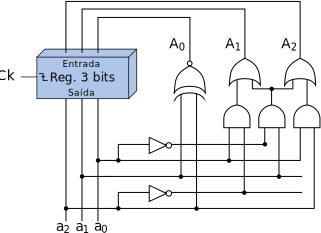
\includegraphics[width=\textwidth]{images/gray_counter_circuit}
\caption{Contador para código de Gray de $3$ bits.}
\label{fig:gray_circuit}
\end{center}
\end{figure}

Note que, na Figura~\ref{fig:gray_circuit}, desprezamos as saídas
$\Not{Q}$. Poderíamos usá-las para economizar portas NOT no
circuito combinacional do cálculo do próximo estado. A
Figura~\ref{fig:gray_circuit_savings} mostra como isso é feito.

\begin{figure}[!htp]
\begin{center}
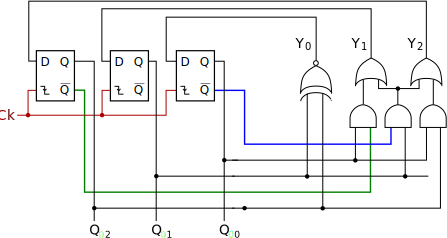
\includegraphics[width=\textwidth]{images/gray_counter_savings}
\caption{Aproveitando as saídas $\Not{Q}$.}
\label{fig:gray_circuit_savings}
\end{center}
\end{figure}

A seguir temos um resumo dos passos usados no projeto deste contador.
Em geral, esses passos podem ser aplicados ao projeto de qualquer
máquina de estados.

\begin{enumerate}
\item Especifique a sequência de estados do contador e
      desenhe o diagrama de estados.
\item Obtenha a tabela de transição a partir do diagrama
      de estados
\item Para cada linha de ativação, obtenha uma expressão
      a partir do diagrama de estados. Para modelos pequenos,
      como os estudados no nosso curso, isso pode ser feito
      por meio de mapas de Karnaugh.
\item Implemente as expressões por meio de lógica combinacional
      e combine com flip-flops para criar o contador.
\end{enumerate}

Note que o projeto de contadores pode ser feito também com
outros flip-flops além daqueles do tipo D. O livro do Floyd
(seção 8-4, 9a ed.) mostra como construir o mesmo contador
usando flip-flops J-K.

\section{Exemplo: Implementação de Contador com Sequência Arbitrária}

Projete um contador para a sequência irregular de contagem
binária mostrada no diagrama de estado da
Figura~\ref{fig:irr_counter_states}. Use flip-flops D.

\begin{figure}[!htp]
\begin{center}
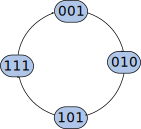
\includegraphics{images/irr_counter_states}
\caption{Diagrama para um contador com sequência arbitrária}
\label{fig:irr_counter_states}
\end{center}
\end{figure}

Há duas maneiras de se implementar este contador. Como
ele possui apenas quatro estados, uma primeira maneira
seria usar um contador de $2$ bits e fazer um circuito
combinacional para transformar a saída, cuja sequência
de estados seria $00$, $01$, $10$, $11$, da seguinte
forma: $00 \rightarrow 001$, $01 \rightarrow 010$,
$10 \rightarrow 101$ e $11 \rightarrow 111$. A segunda
maneira, a qual demonstraremos a seguir, é implementar
um contador síncrono de $3$ bits que
transita diretamente entre esses quatro estados.

\textbf{Passo 1}: já nos foi dado o diagrama de estados,
portanto nada mais há a fazer neste passo.

\textbf{Passo 2}: na Tabela~\ref{tab:irr_counter} temos
a tabela de transição desenvolvida a partir do diagrama
de estado.

\begin{table}[!htp]
\begin{center}
\caption{Tabela de transição.}
\label{tab:irr_counter}
\begin{tabular}{|ccc||ccc|}
\hline
\multicolumn{3}{|c||}{atual} & \multicolumn{3}{c|}{próximo} \\
  $Q_2$  &  $Q_1$  &  $Q_0$  &  $Y_2$  &  $Y_1$  &  $Y_0$   \\
\hline
    0    &    0    &    1    &    0    &    1    &    0     \\
    0    &    1    &    0    &    1    &    0    &    1     \\
    1    &    0    &    1    &    1    &    1    &    1     \\
    1    &    1    &    1    &    0    &    0    &    1     \\
\hline
\end{tabular}
\end{center}
\end{table}

\textbf{Passo 3:} determinação e otimização de expressões.
Das tabelas-verdade para $Y_0$, $Y_1$ e $Y_2$ obtemos os
mapas de Karnaugh da Figura~\ref{fig:irr_counter_karnaugh}.
Note que há várias células preenchidas com um X, que
correspondem os estados para $Q_2$, $Q_1$ e $Q_0$ que nunca
serão alcançados --- neste caso, os estados $000$, $011$, $100$ e
$110$. Uma célula preenchida com um X (também
chamada de \emph{don't care}) pode ser agrupada junto com
um ou mais $1$s, \textbf{desde que ela sirva para simplificar a
expressão}.

\def\L{\raisebox{-4pt}}

\begin{figure}[!htp]
\begin{center}
\begin{minipage}{0.4\textwidth}
\begin{center}
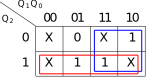
\includegraphics{images/kmap_irr_counter_y0}\\[12pt]
(a) Mapa para $Y_0$
\end{center}
\end{minipage}%
%
\hfill%
%
\begin{minipage}{0.4\textwidth}
\begin{center}
\includegraphics{images/kmap_irr_counter_y1}\\[12pt]
(a) Mapa para $Y_1$
\end{center}
\end{minipage}%

\begin{minipage}{0.4\textwidth}
\begin{center}
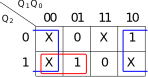
\includegraphics{images/kmap_irr_counter_y2}\\[12pt]
(a) Mapa para $Y_2$
\end{center}
\end{minipage}

\caption{Mapas de Karnaugh para o próximo estado do contador irregular.}
\label{fig:irr_counter_karnaugh}
\end{center}
\end{figure}

Com os agrupamentos mostrados na Figura~\ref{fig:irr_counter_karnaugh},
obtemos as seguintes expressões:
\begin{itemize}
\item $Y_0 = Q_1 + Q_2$
\item $Y_1 = \Not{Q_1}$
\item $Y_2 = \Not{Q_0} + \Not{Q_1} \, Q_2$
\end{itemize}

\textbf{Passo 4}: a implementação do contador irregular é
mostrada na Figura~\ref{fig:irr_counter_circuit}.

\begin{figure}[!htp]
\begin{center}
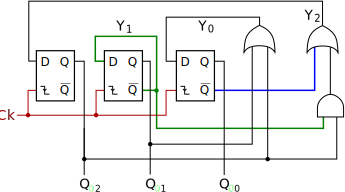
\includegraphics{images/irr_counter_circuit}
\caption{Implementação do contador irregular.}
\label{fig:irr_counter_circuit}
\end{center}
\end{figure}

\section{Exercícios}

Faça os exercícios 14 e 15 do capítulo 8 do livro do Floyd.
Nos exercícios 16, 17 e 18 use flip-flops D em vez de flip-flops J-K.

\begin{thebibliography}{9}
\bibitem{Floyd1997}
  FLOYD, Thomas L.
  \emph{Sistemas Digitais: Fundamentos e Aplicações}.
  Editora Bookman,
  9\ba Edição,
  2007.
\end{thebibliography}

\end{document}
